
\documentclass[11pt,a4paper]{article}
\usepackage[T1]{fontenc}
\usepackage[utf8]{inputenc}
\usepackage[polish]{babel}
\usepackage{lmodern}
\usepackage{geometry}
\geometry{margin=2.2cm}
\usepackage{graphicx}
\usepackage{subcaption}
\usepackage{booktabs}
\usepackage{amsmath,amssymb}
\usepackage{xcolor}
\usepackage{listings}
\lstdefinestyle{cppstyle}{
  language=C++,
  basicstyle=\ttfamily\footnotesize,
  keywordstyle=\color{blue!60!black}\bfseries,
  commentstyle=\color{gray!70}\itshape,
  stringstyle=\color{green!40!black},
  numbers=left,
  numberstyle=\tiny\color{gray},
  stepnumber=1,
  numbersep=8pt,
  showstringspaces=false,
  tabsize=2,
  frame=single,
  breaklines=true
}
\title{Sprawozdanie: Analiza wybranych algorytmów sortowania\\
{\large (Insertion Sort, Insertion Sort Pairs, Merge Sort, Merge Sort 3, Heap Sort, Heap Sort 3)}}
\author{}
\date{\today}

\begin{document}
\maketitle

\section{Wstęp}
Celem pracy była analiza sześciu zaimplementowanych algorytmów sortowania: \emph{Insertion Sort}, jego modyfikacji wstawiającej elementy parami (\emph{Insertion Sort Pairs}), \emph{Merge Sort} (klasyczny dwudzielny), jego wariantu trójdzielnego (\emph{Merge Sort 3}), a także \emph{Heap Sort} w wersji binarnej i ternarnej.
Dla każdego algorytmu zliczano liczbę elementarnych operacji (przestawień), a następnie zebrano wyniki dla rozmiarów tablic $n=10,\dots,1999$. Generator danych używa stałego ziarna \texttt{srand(10)}, dzięki czemu każde uruchomienie daje identyczne wektory wejściowe.
Wszystkie pomiary wykonano tym samym programem testującym.

\begin{figure}[h]
  \centering
  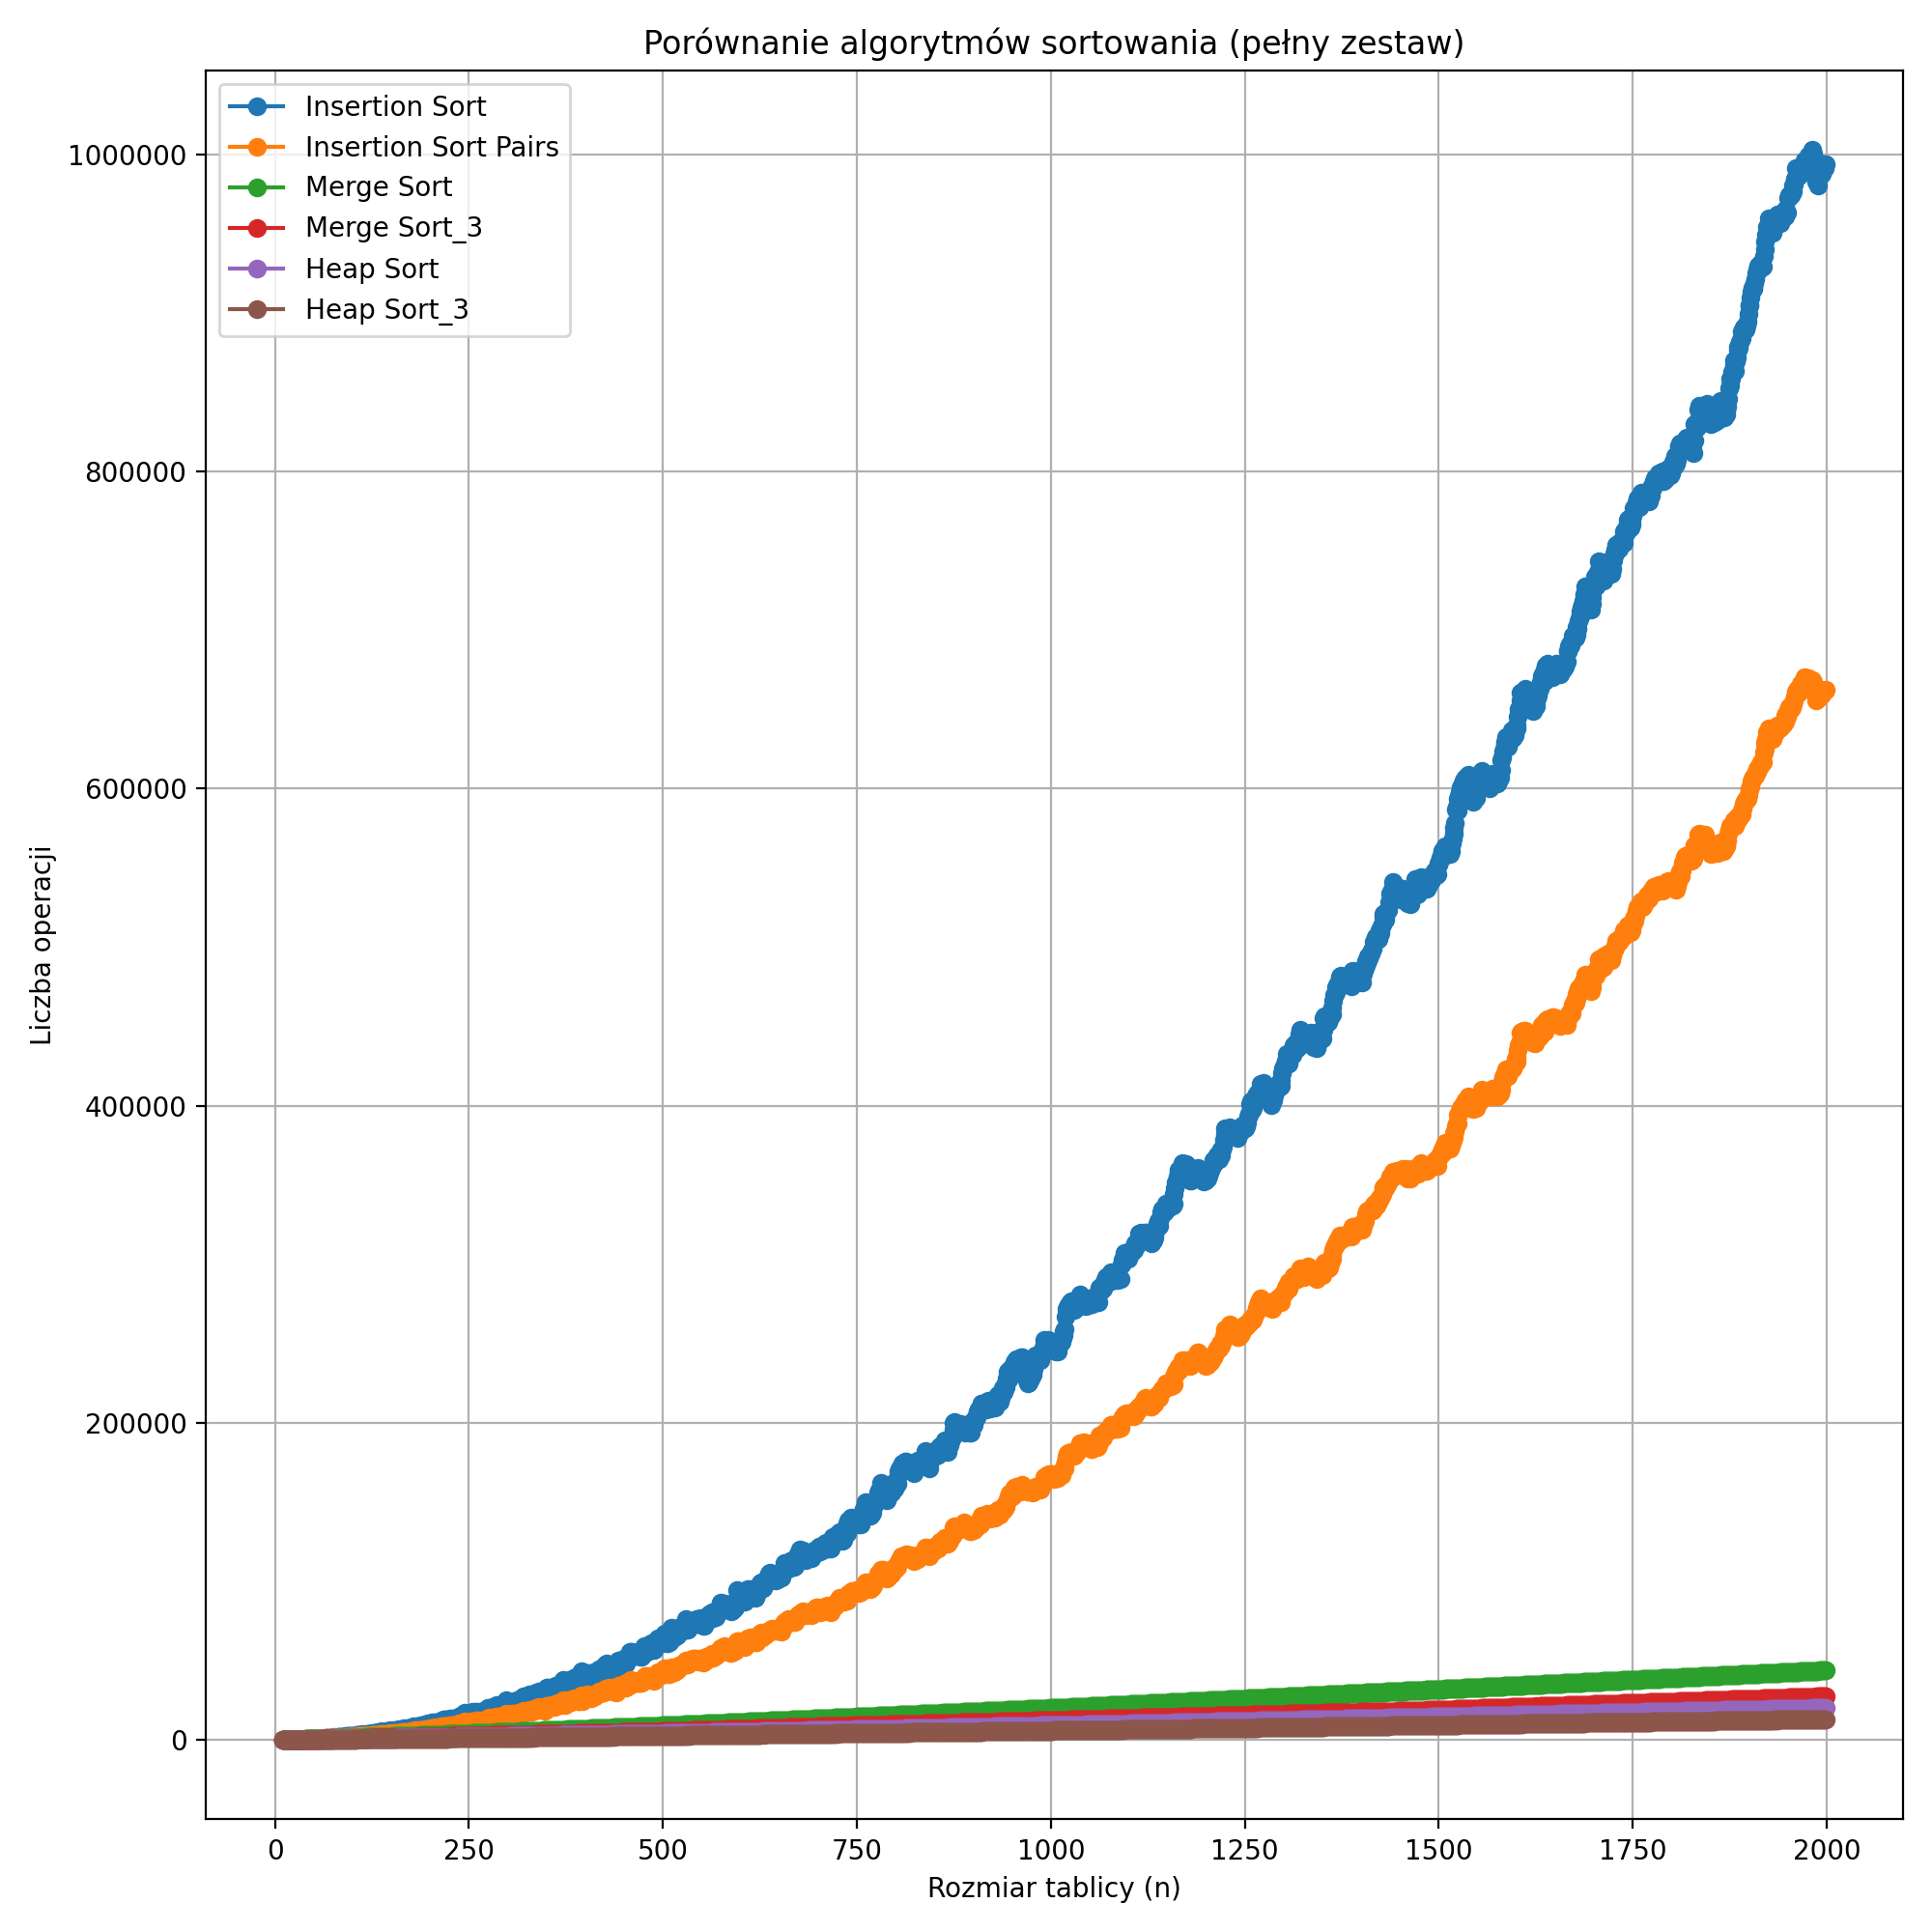
\includegraphics[width=.68\textwidth]{operations_all.png}
  \caption{Liczba operacji w funkcji rozmiaru wejścia --- porównanie wszystkich metod.}
  \label{fig:all}
\end{figure}

\section{Opis algorytmów}
\begin{itemize}
  \item \textbf{Insertion Sort} --- sortowanie przez wstawianie, złożoność średnia i pesymistyczna $O(n^2)$. Dobre dla prawie posortowanych danych.
  \item \textbf{Insertion Sort Pairs} --- modyfikacja, w której do listy wstawia się jednocześnie parę elementów (po wcześniejszym ich uporządkowaniu). Teoretycznie nadal $O(n^2)$, w praktyce redukuje liczbę przesunięć.
  \item \textbf{Merge Sort} --- klasyczne dziel i zwyciężaj; rekurencyjnie dzieli tablicę na dwie połowy. Złożoność $O(n\log n)$.
  \item \textbf{Merge Sort 3} --- wariant dzielący na trzy części i łączący. Teoretycznie również $O(n\log n)$, lecz z inną stałą.
  \item \textbf{Heap Sort (binarny)} --- budowa kopca. Złożoność $O(n\log n)$.
  \item \textbf{Heap Sort 3} --- analogiczny do wersji binarnej, lecz kopiec ternarny (trzech potomków); mniejsza wysokość kopca, ale droższe pojedyncze \texttt{heapify}.
\end{itemize}

\section{Najciekawsze fragmenty kodu: \emph{Merge Sort}}
Poniżej pokazano dwa kluczowe fragmenty: funkcję sklejającą i rekurencyjne dzielenie. Pierwsza z nich odpowiada za liniowe łączenie dwóch posortowanych list (lewego i prawego) w jeden przedział tablicy wejściowej. Zmienna \texttt{number} służy jako licznik operacji przestawień wykorzystywany w analizie.
\medskip

\noindent\textbf{Funkcja \texttt{merge} (fragment z \texttt{merge\_sort.cpp}):}
\begin{lstlisting}[style=cppstyle,caption={Sklejanie dwóch przedziałów w Merge Sort.},label={lst:merge}]
int merge(int list[], int begin, int middle, int end, int number) {
    int len_left = middle - begin + 1;
    int len_right = end - middle;
    int left_list[len_left];
    int right_list[len_right];
    for (int i = begin; i < begin+len_left; i++) {
        left_list[i-begin] = list[i];
        number++;
    }
    for (int i = middle; i < middle+len_right; i++) {
        right_list[i-middle] = list[i+1];
        number++;
    }
    int left_index = 0;
    right_index = 0;
    for (int i = begin; i <= end; i++) {
    	if ((left_index < len_left and left_list[left_index] <= right_list[right_index]) or right_index >= len_right){
    		list[i] = left_list[left_index];
    		left_index++;
    		number++;
    		
    	}
    	else {
    		list[i] = right_list[right_index]; 
    		right_index++;
    		number++;
    		
    	}
    	
    }
    return number;
}
\end{lstlisting}

\noindent\textbf{Podział i wywołania rekurencyjne:}
\begin{lstlisting}[style=cppstyle,caption={Rekurencyjny podział i łączenie.},label={lst:mergesort}]
int merge_sort(int list[], int begin, int end, int number) {
    if (begin < end) {
        int middle = floor((begin+end)/2);
        number = merge_sort(list, begin, middle, number);
        number = merge_sort(list, middle+1, end, number);
        number = merge(list, begin, middle, end, number);
    }
    return number;
}
\end{lstlisting}


\section{Porównania i wyniki}
Na rys.~\ref{fig:all} widać wyraźny rozjazd między metodami $O(n^2)$ (\emph{Insertion}) i $O(n\log n)$ (rodzina \emph{Merge}/\emph{Heap}). Aby lepiej zobaczyć indywidualne przebiegi, poniżej zamieszczono mini-wykresy (oryginały zapisane w plikach PNG).

\begin{figure}[h]
  \centering
  \begin{subfigure}{.32\textwidth}
    \centering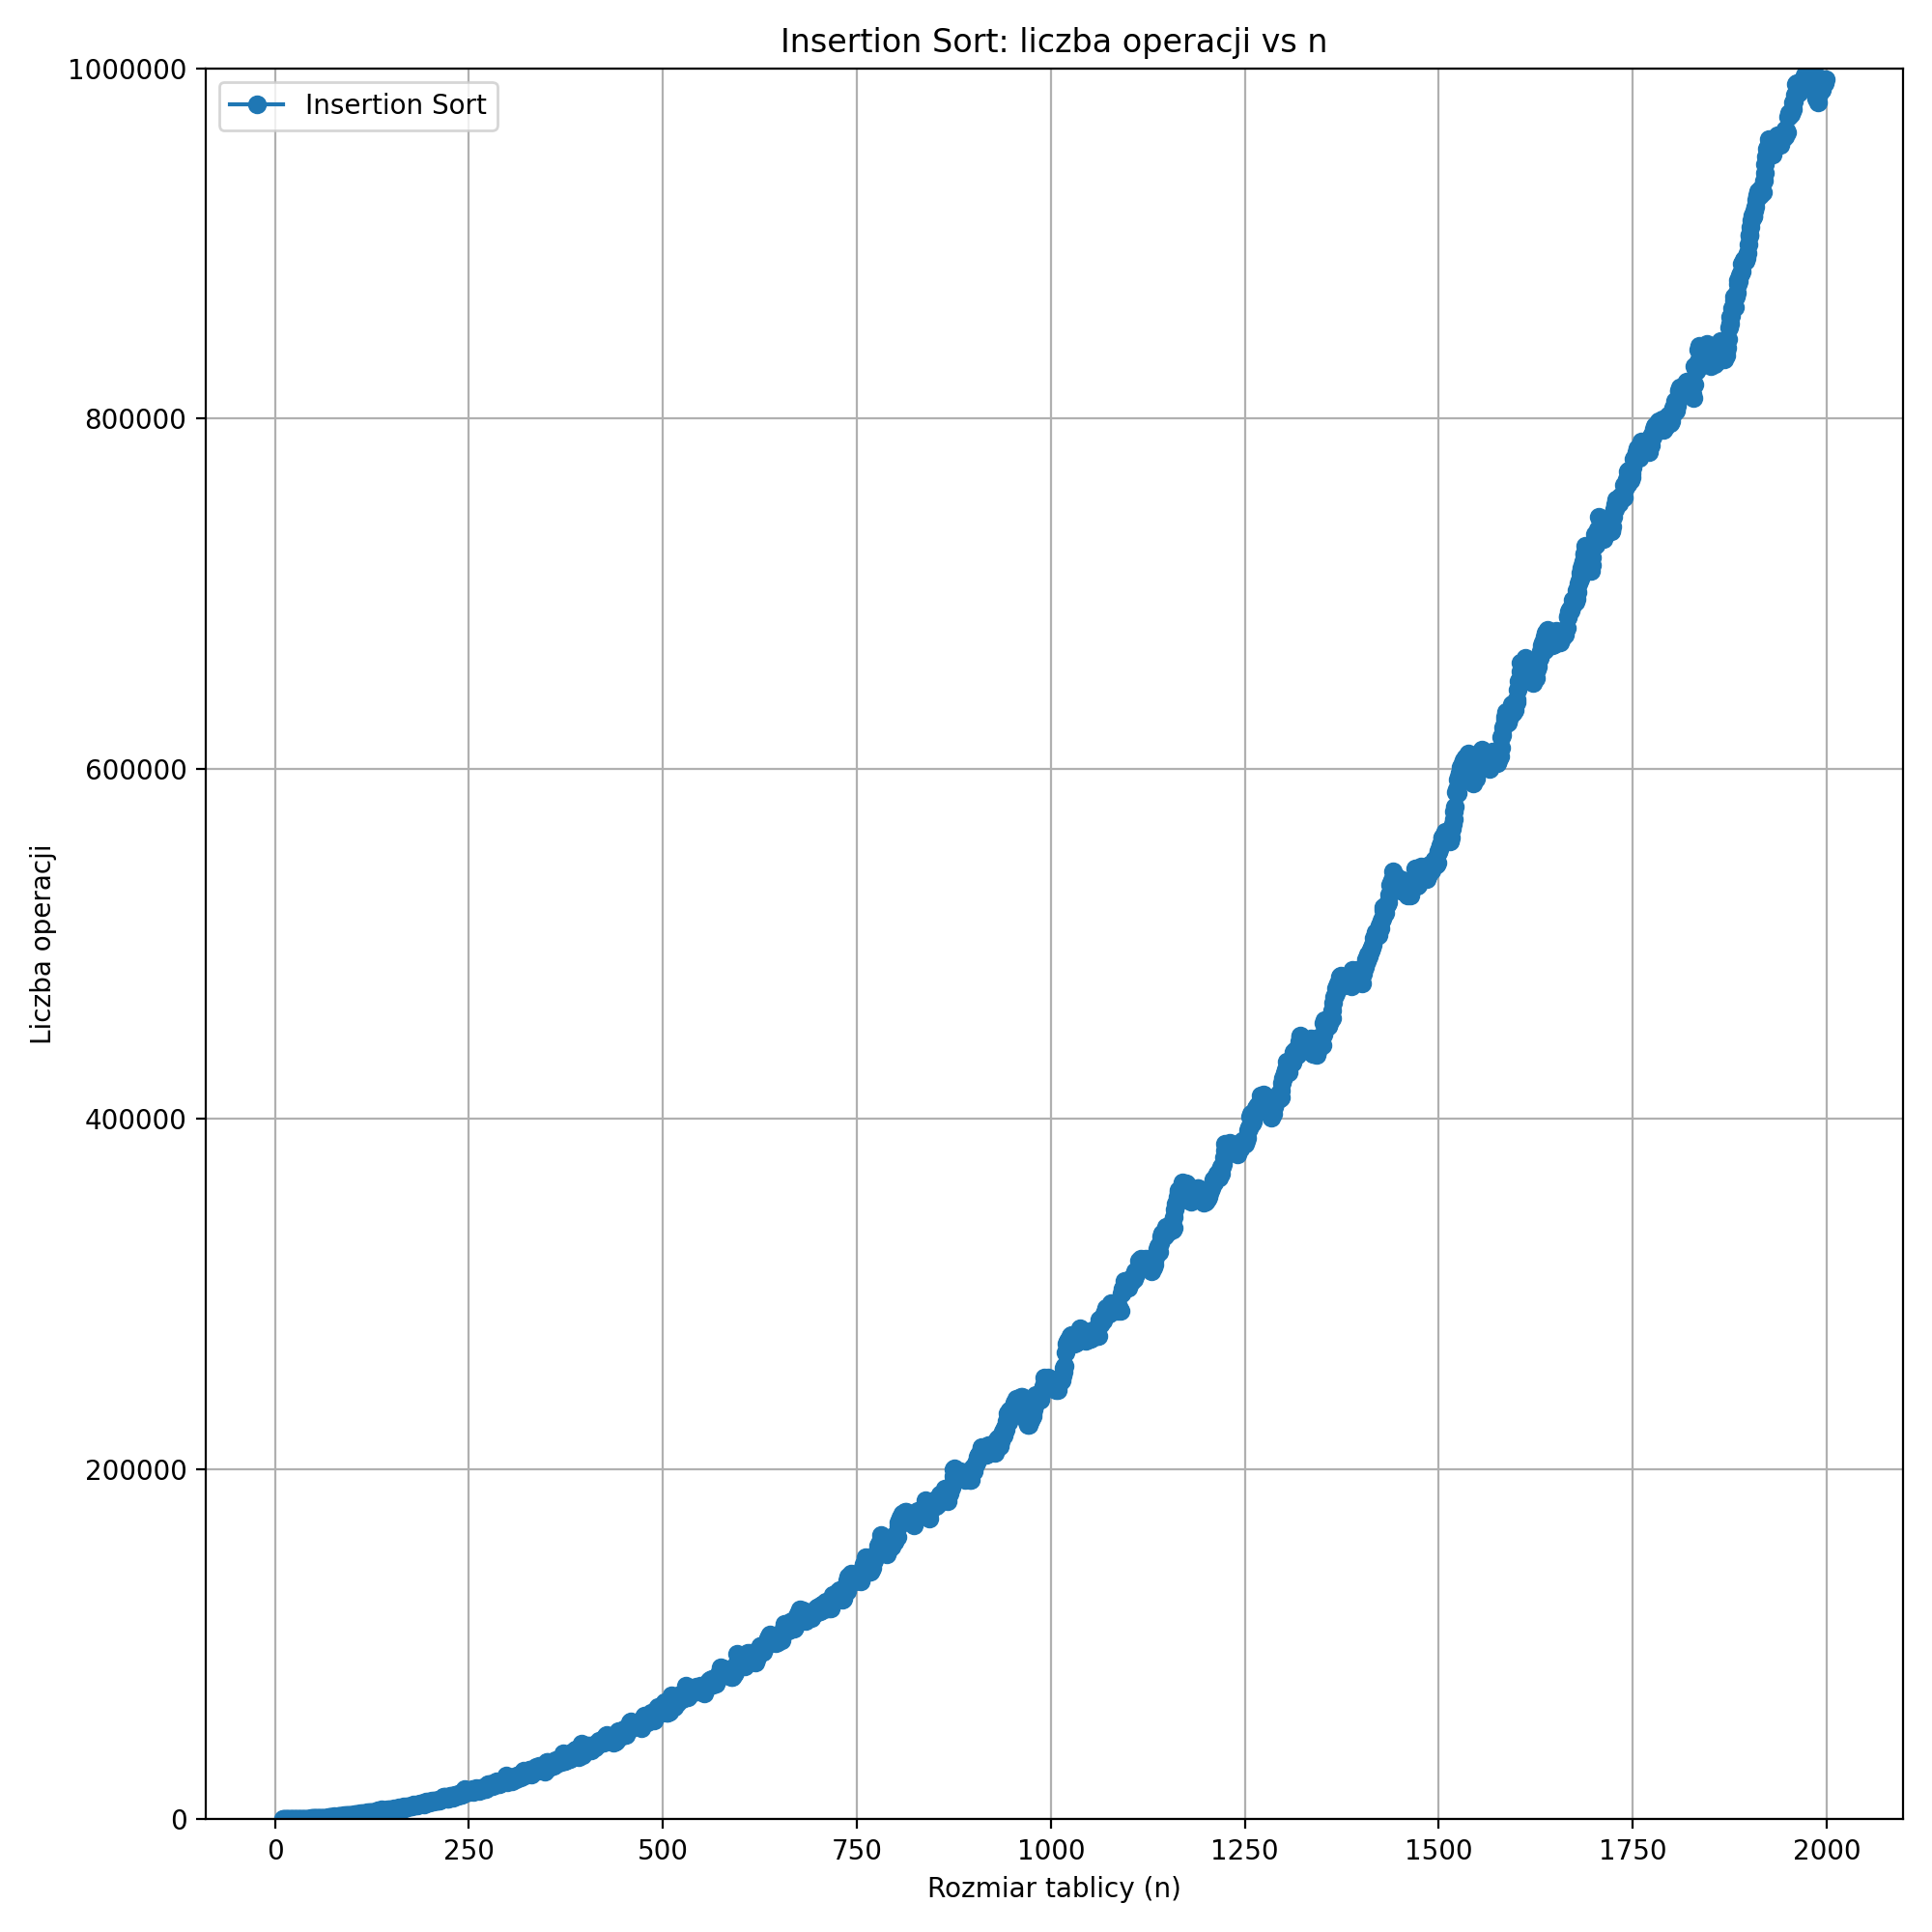
\includegraphics[width=\linewidth]{insertion_sort.png}
    \caption{Insertion Sort}
  \end{subfigure}
  \begin{subfigure}{.32\textwidth}
    \centering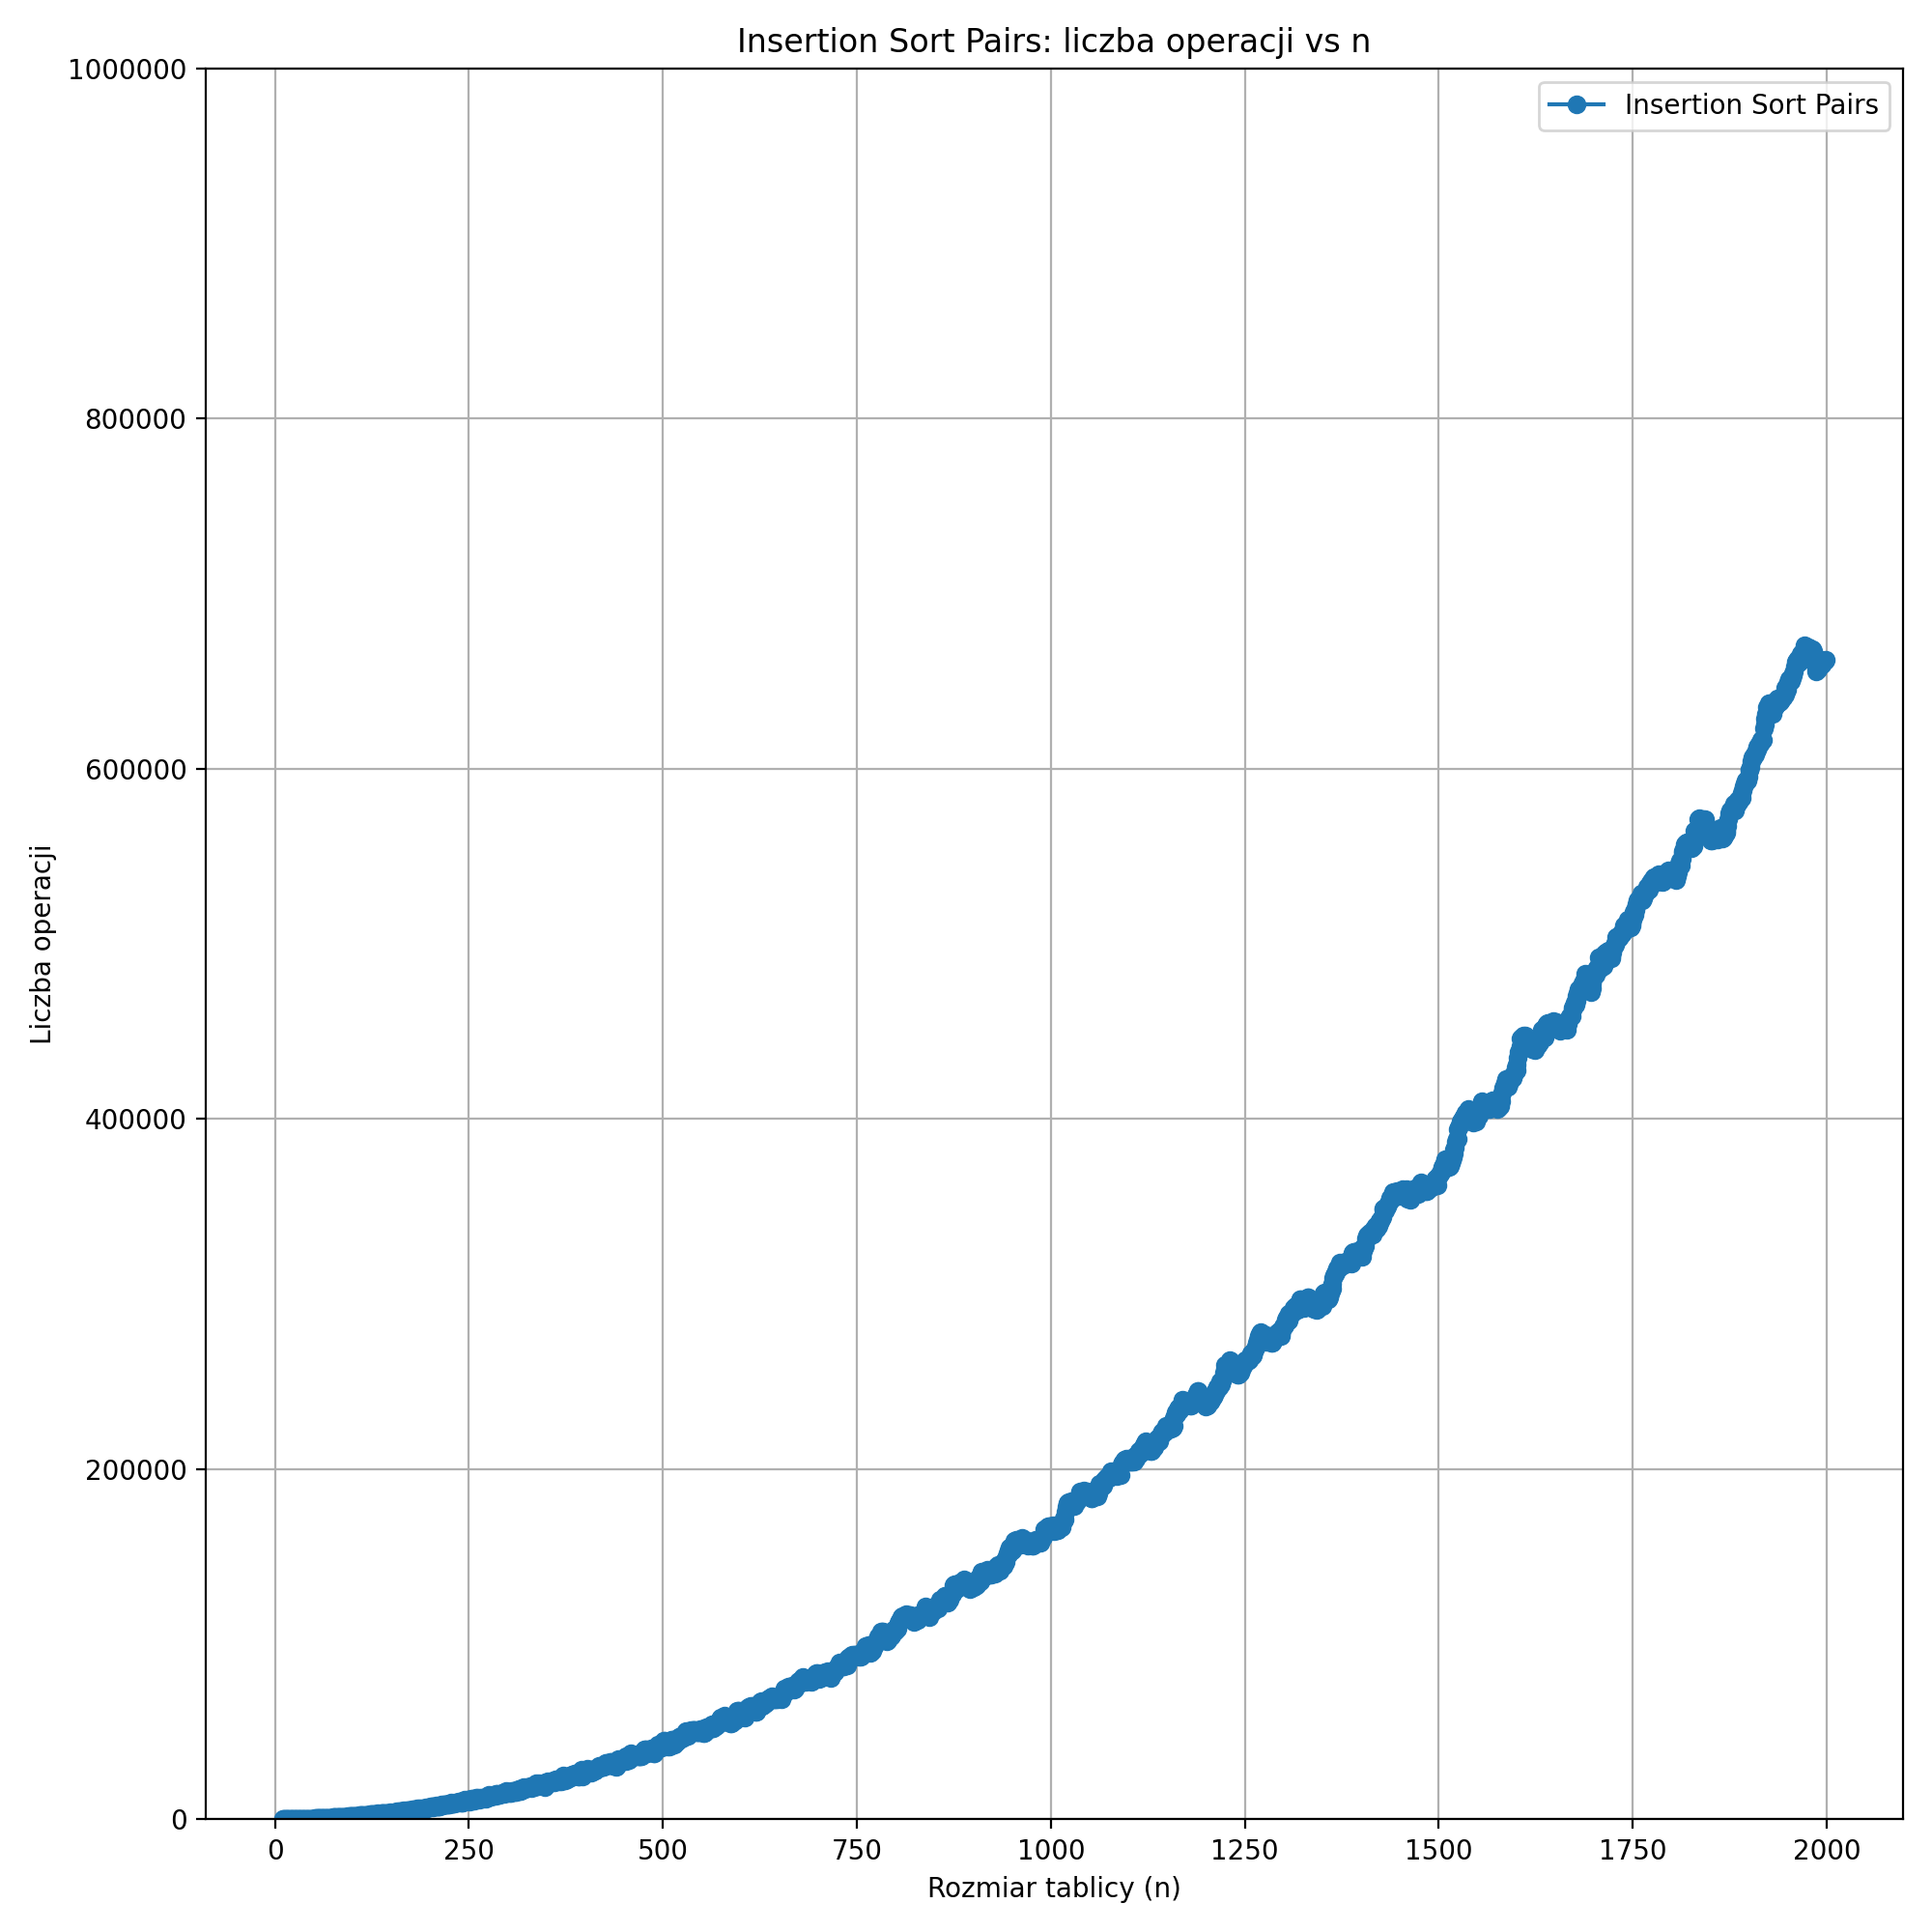
\includegraphics[width=\linewidth]{insertion_sort_pairs.png}
    \caption{Insertion Sort Pairs}
  \end{subfigure}
  \begin{subfigure}{.32\textwidth}
    \centering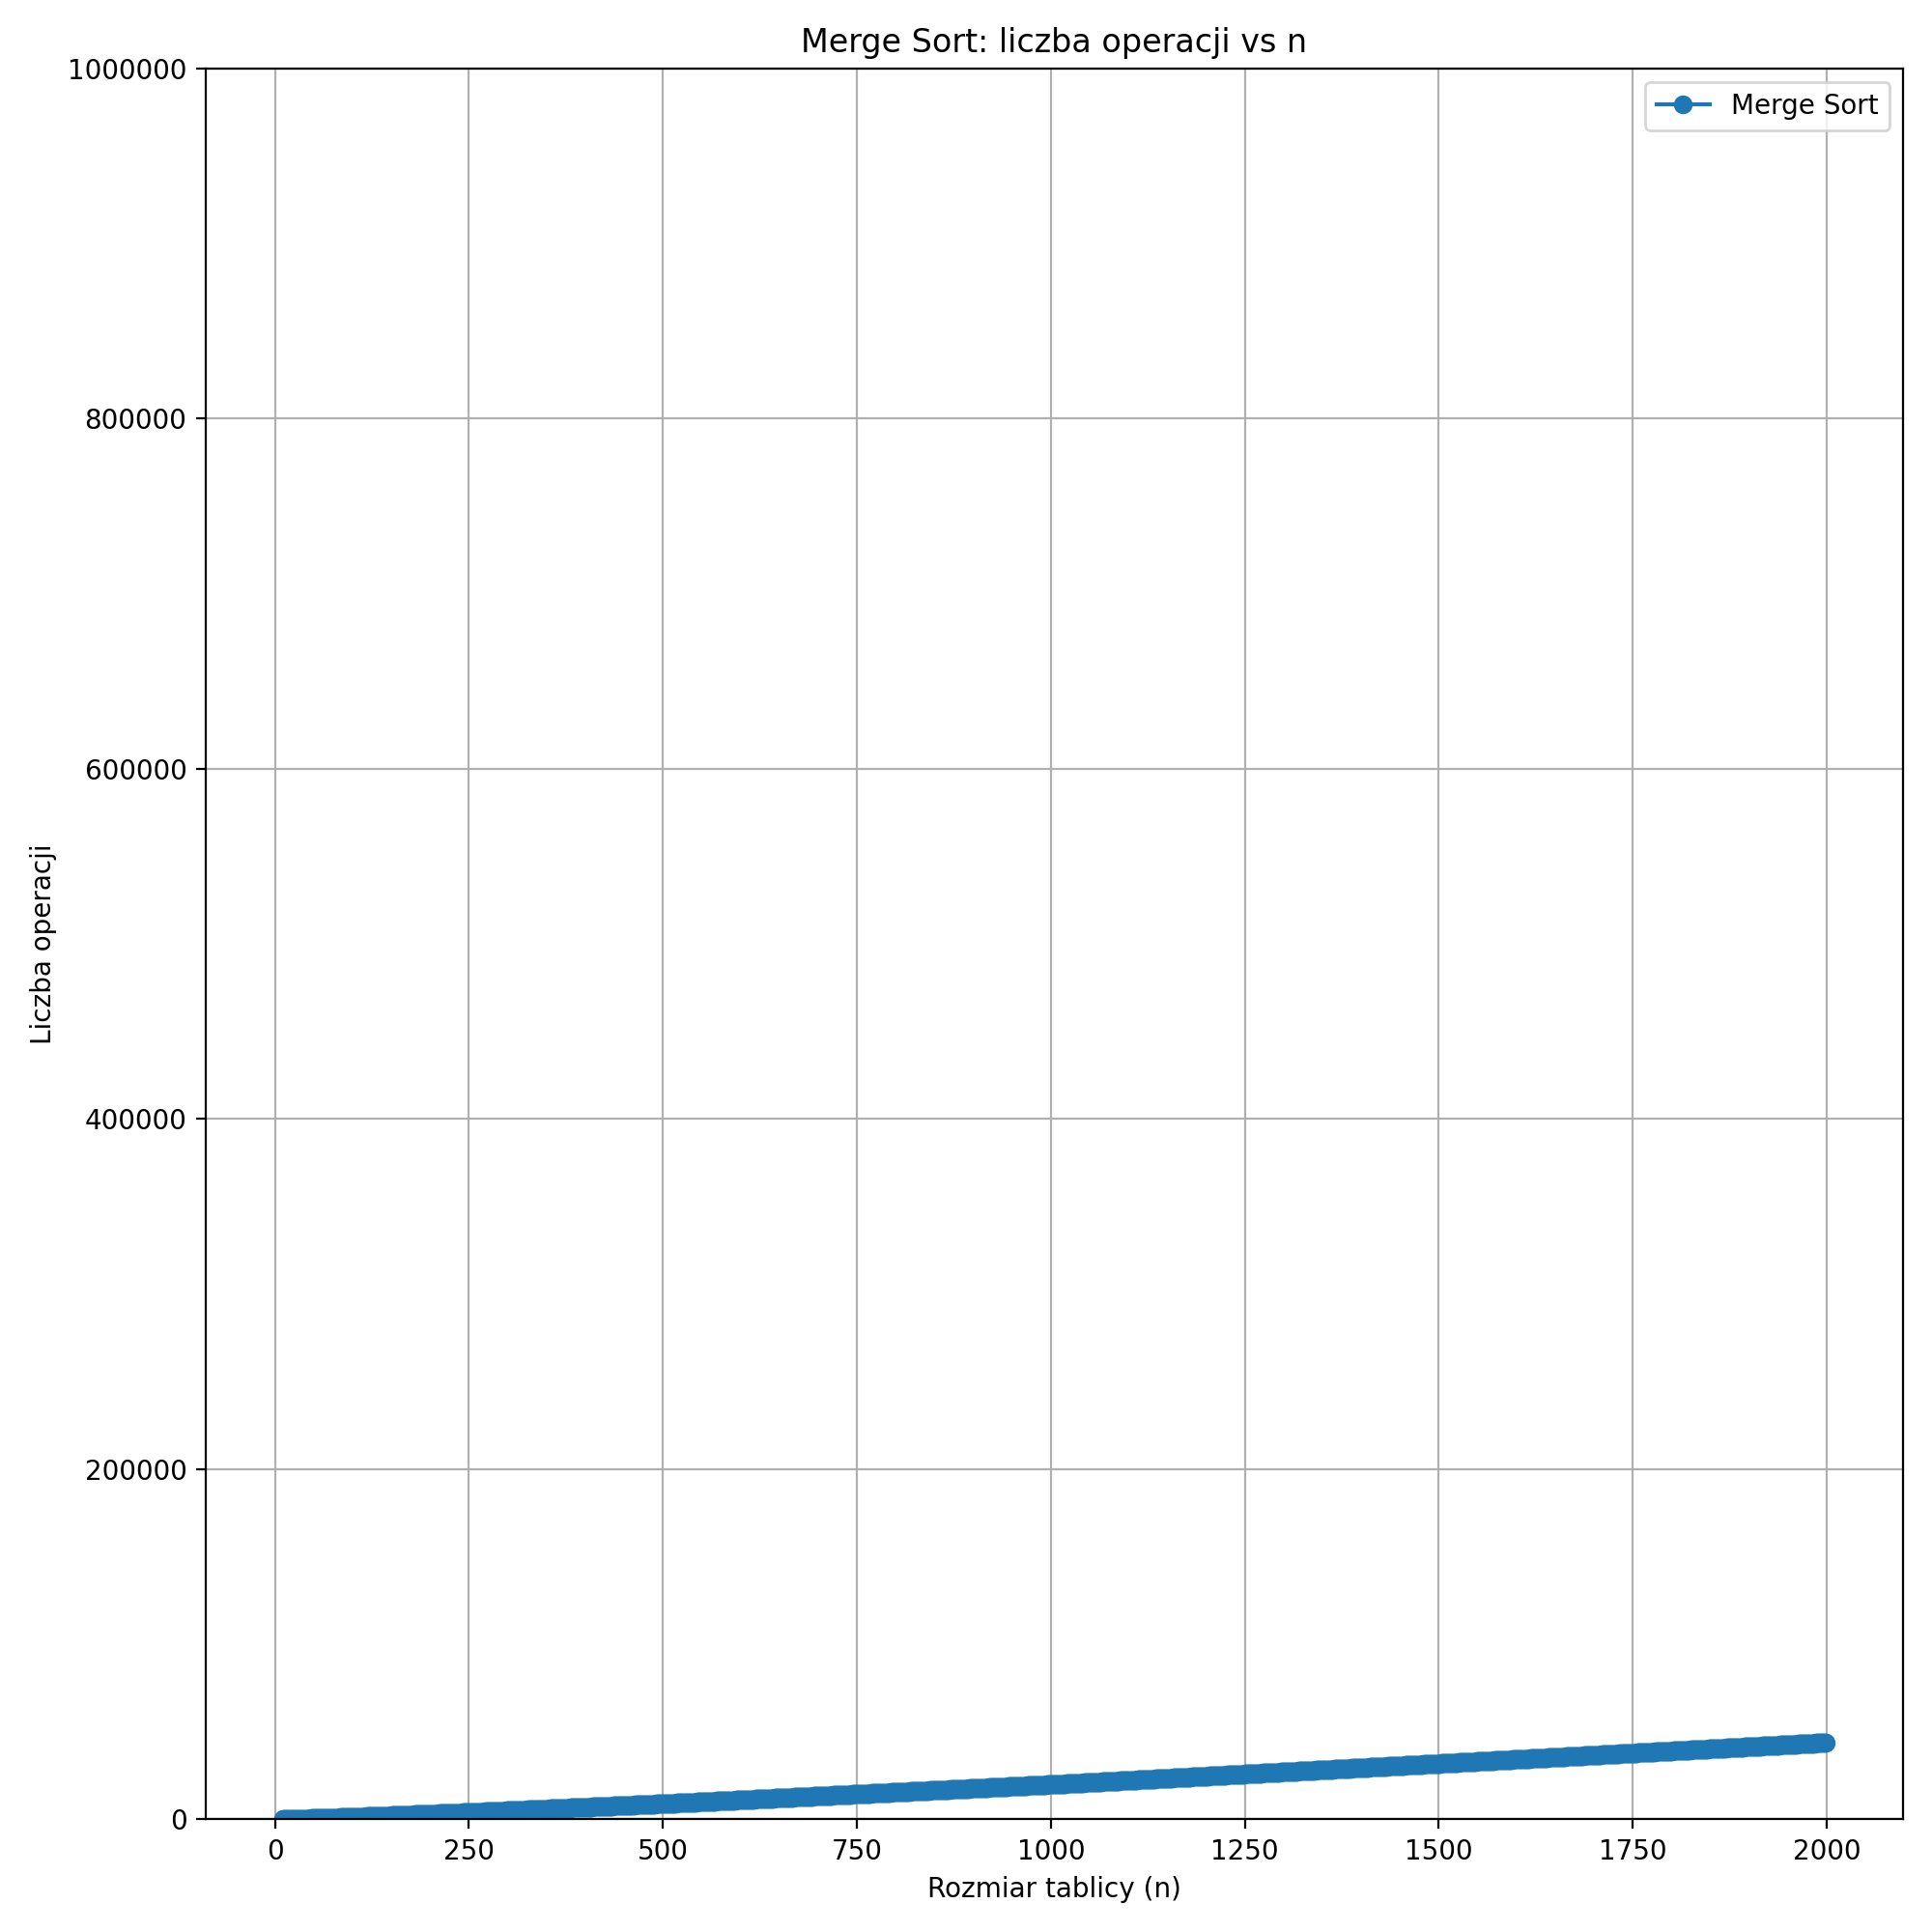
\includegraphics[width=\linewidth]{merge_sort.png}
    \caption{Merge Sort}
  \end{subfigure}

  \begin{subfigure}{.32\textwidth}
    \centering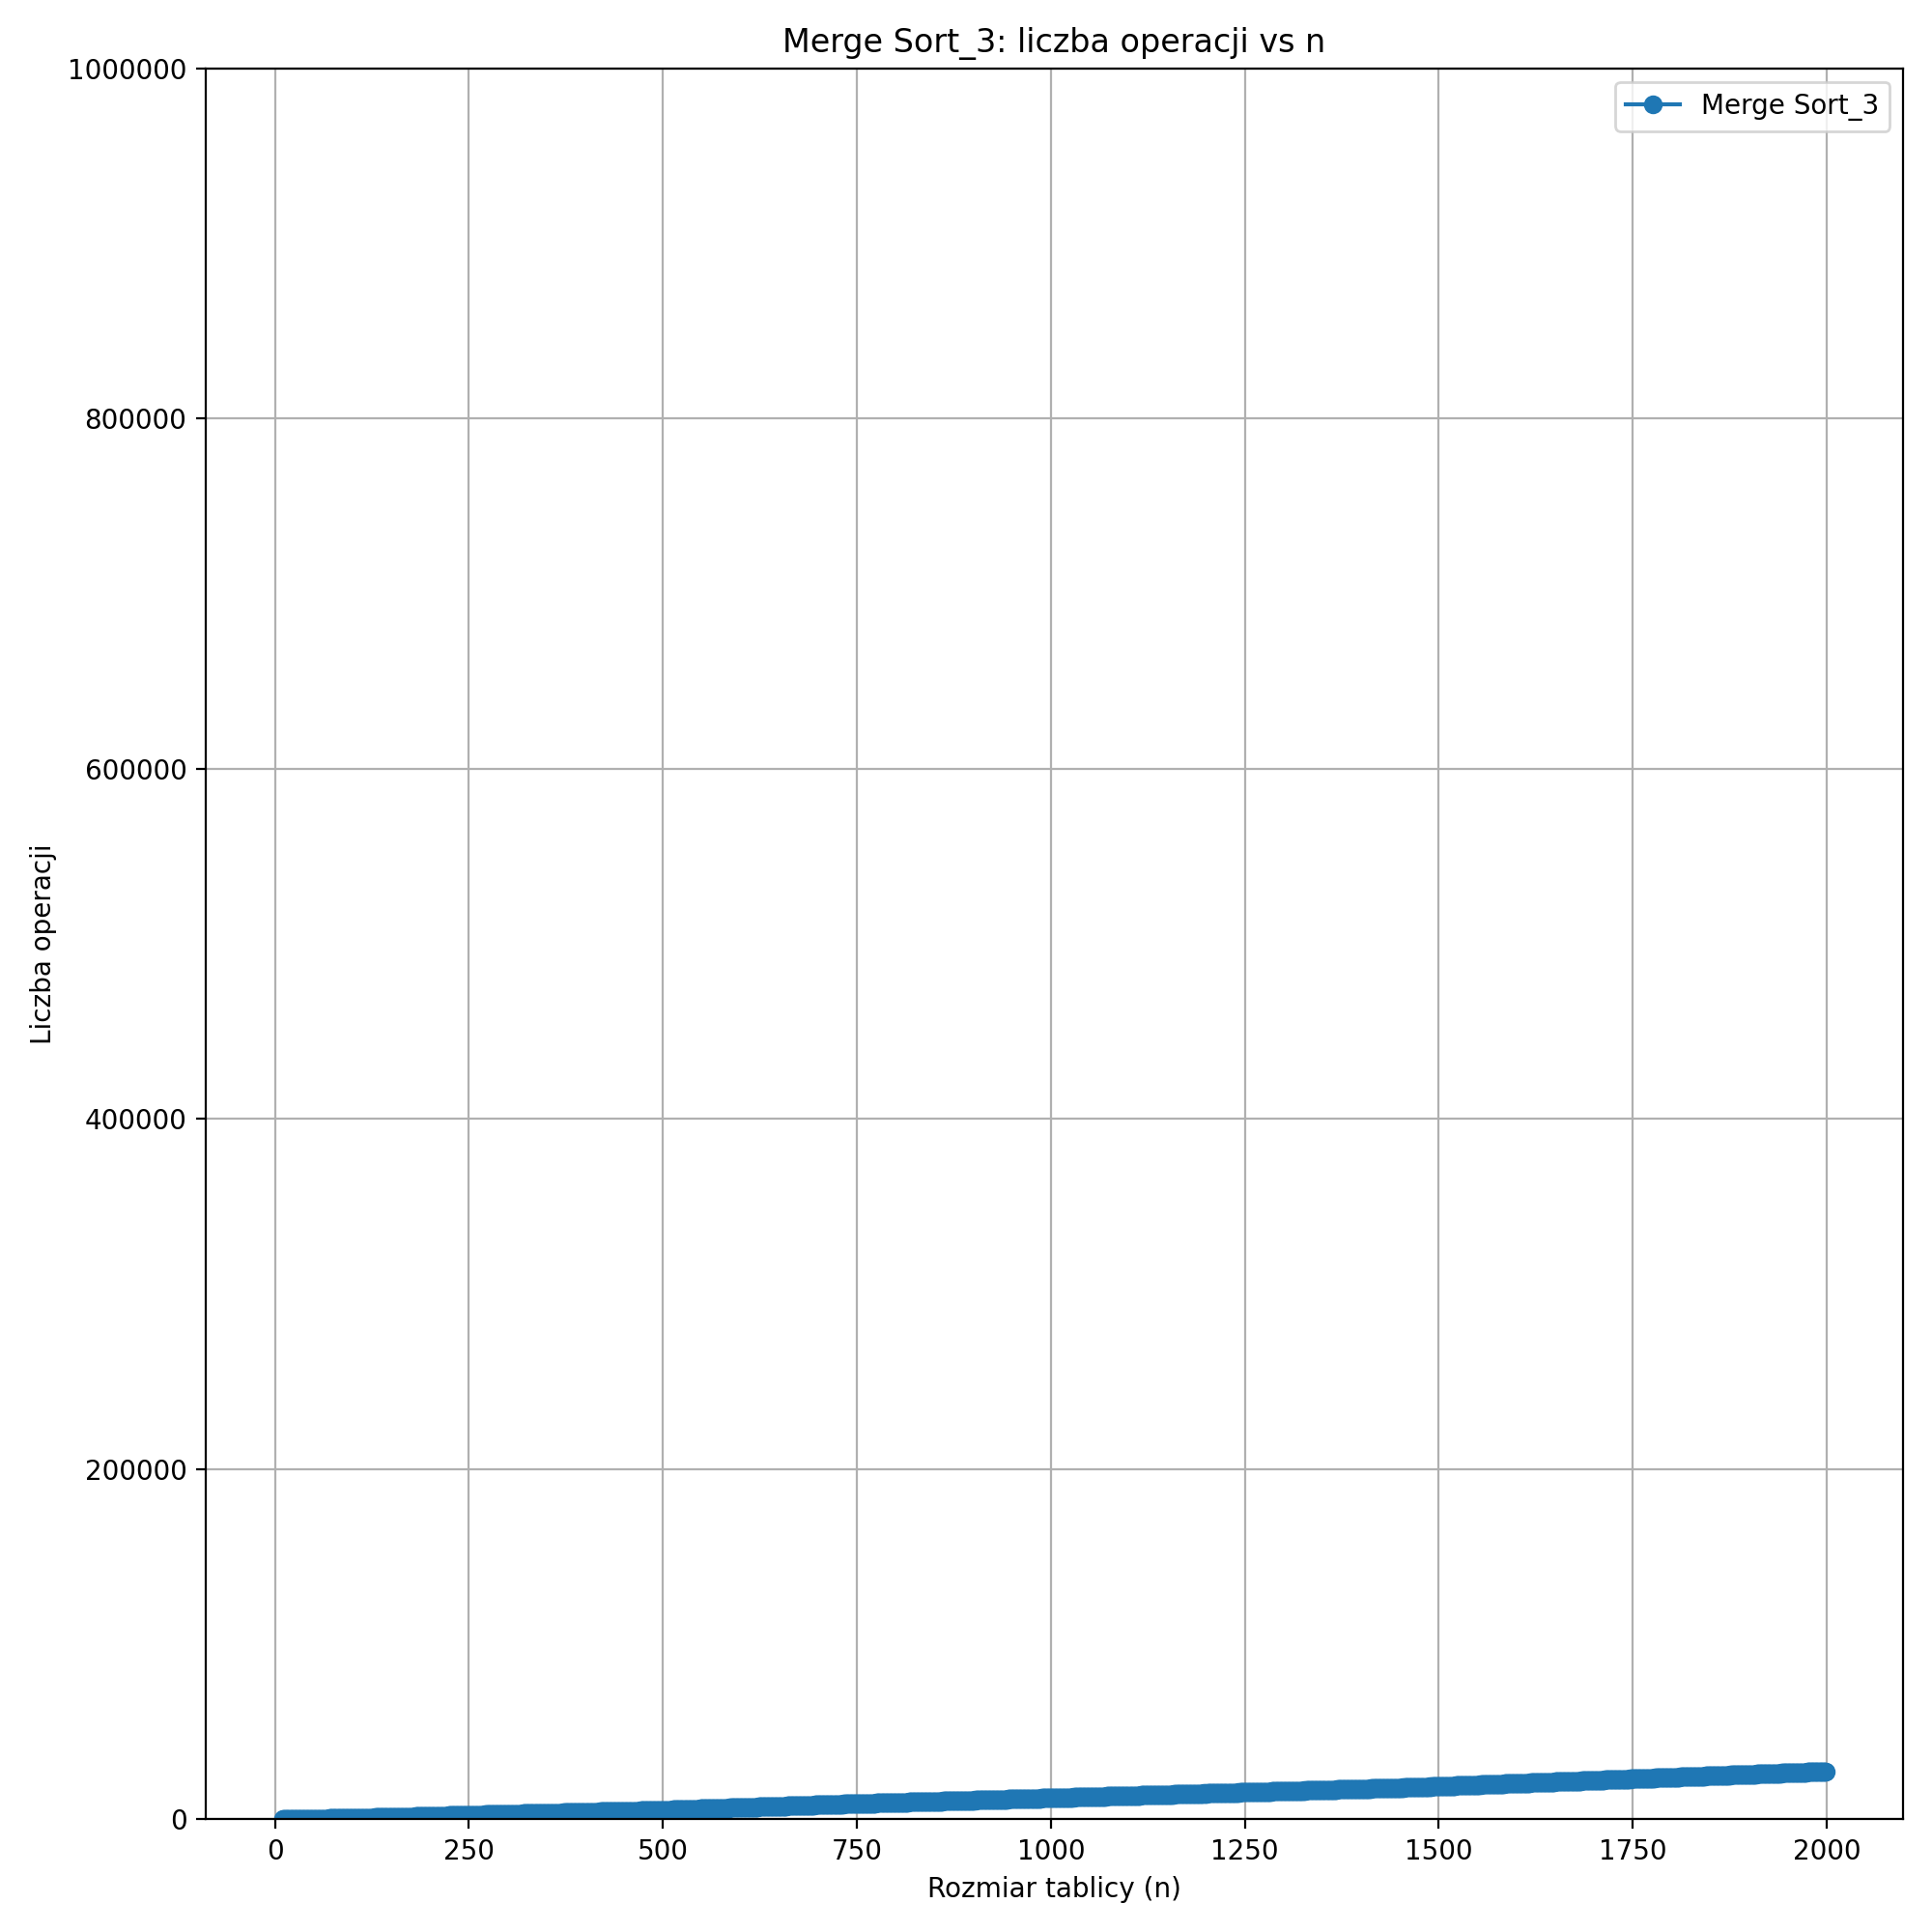
\includegraphics[width=\linewidth]{merge_sort_3.png}
    \caption{Merge Sort 3}
  \end{subfigure}
  \begin{subfigure}{.32\textwidth}
    \centering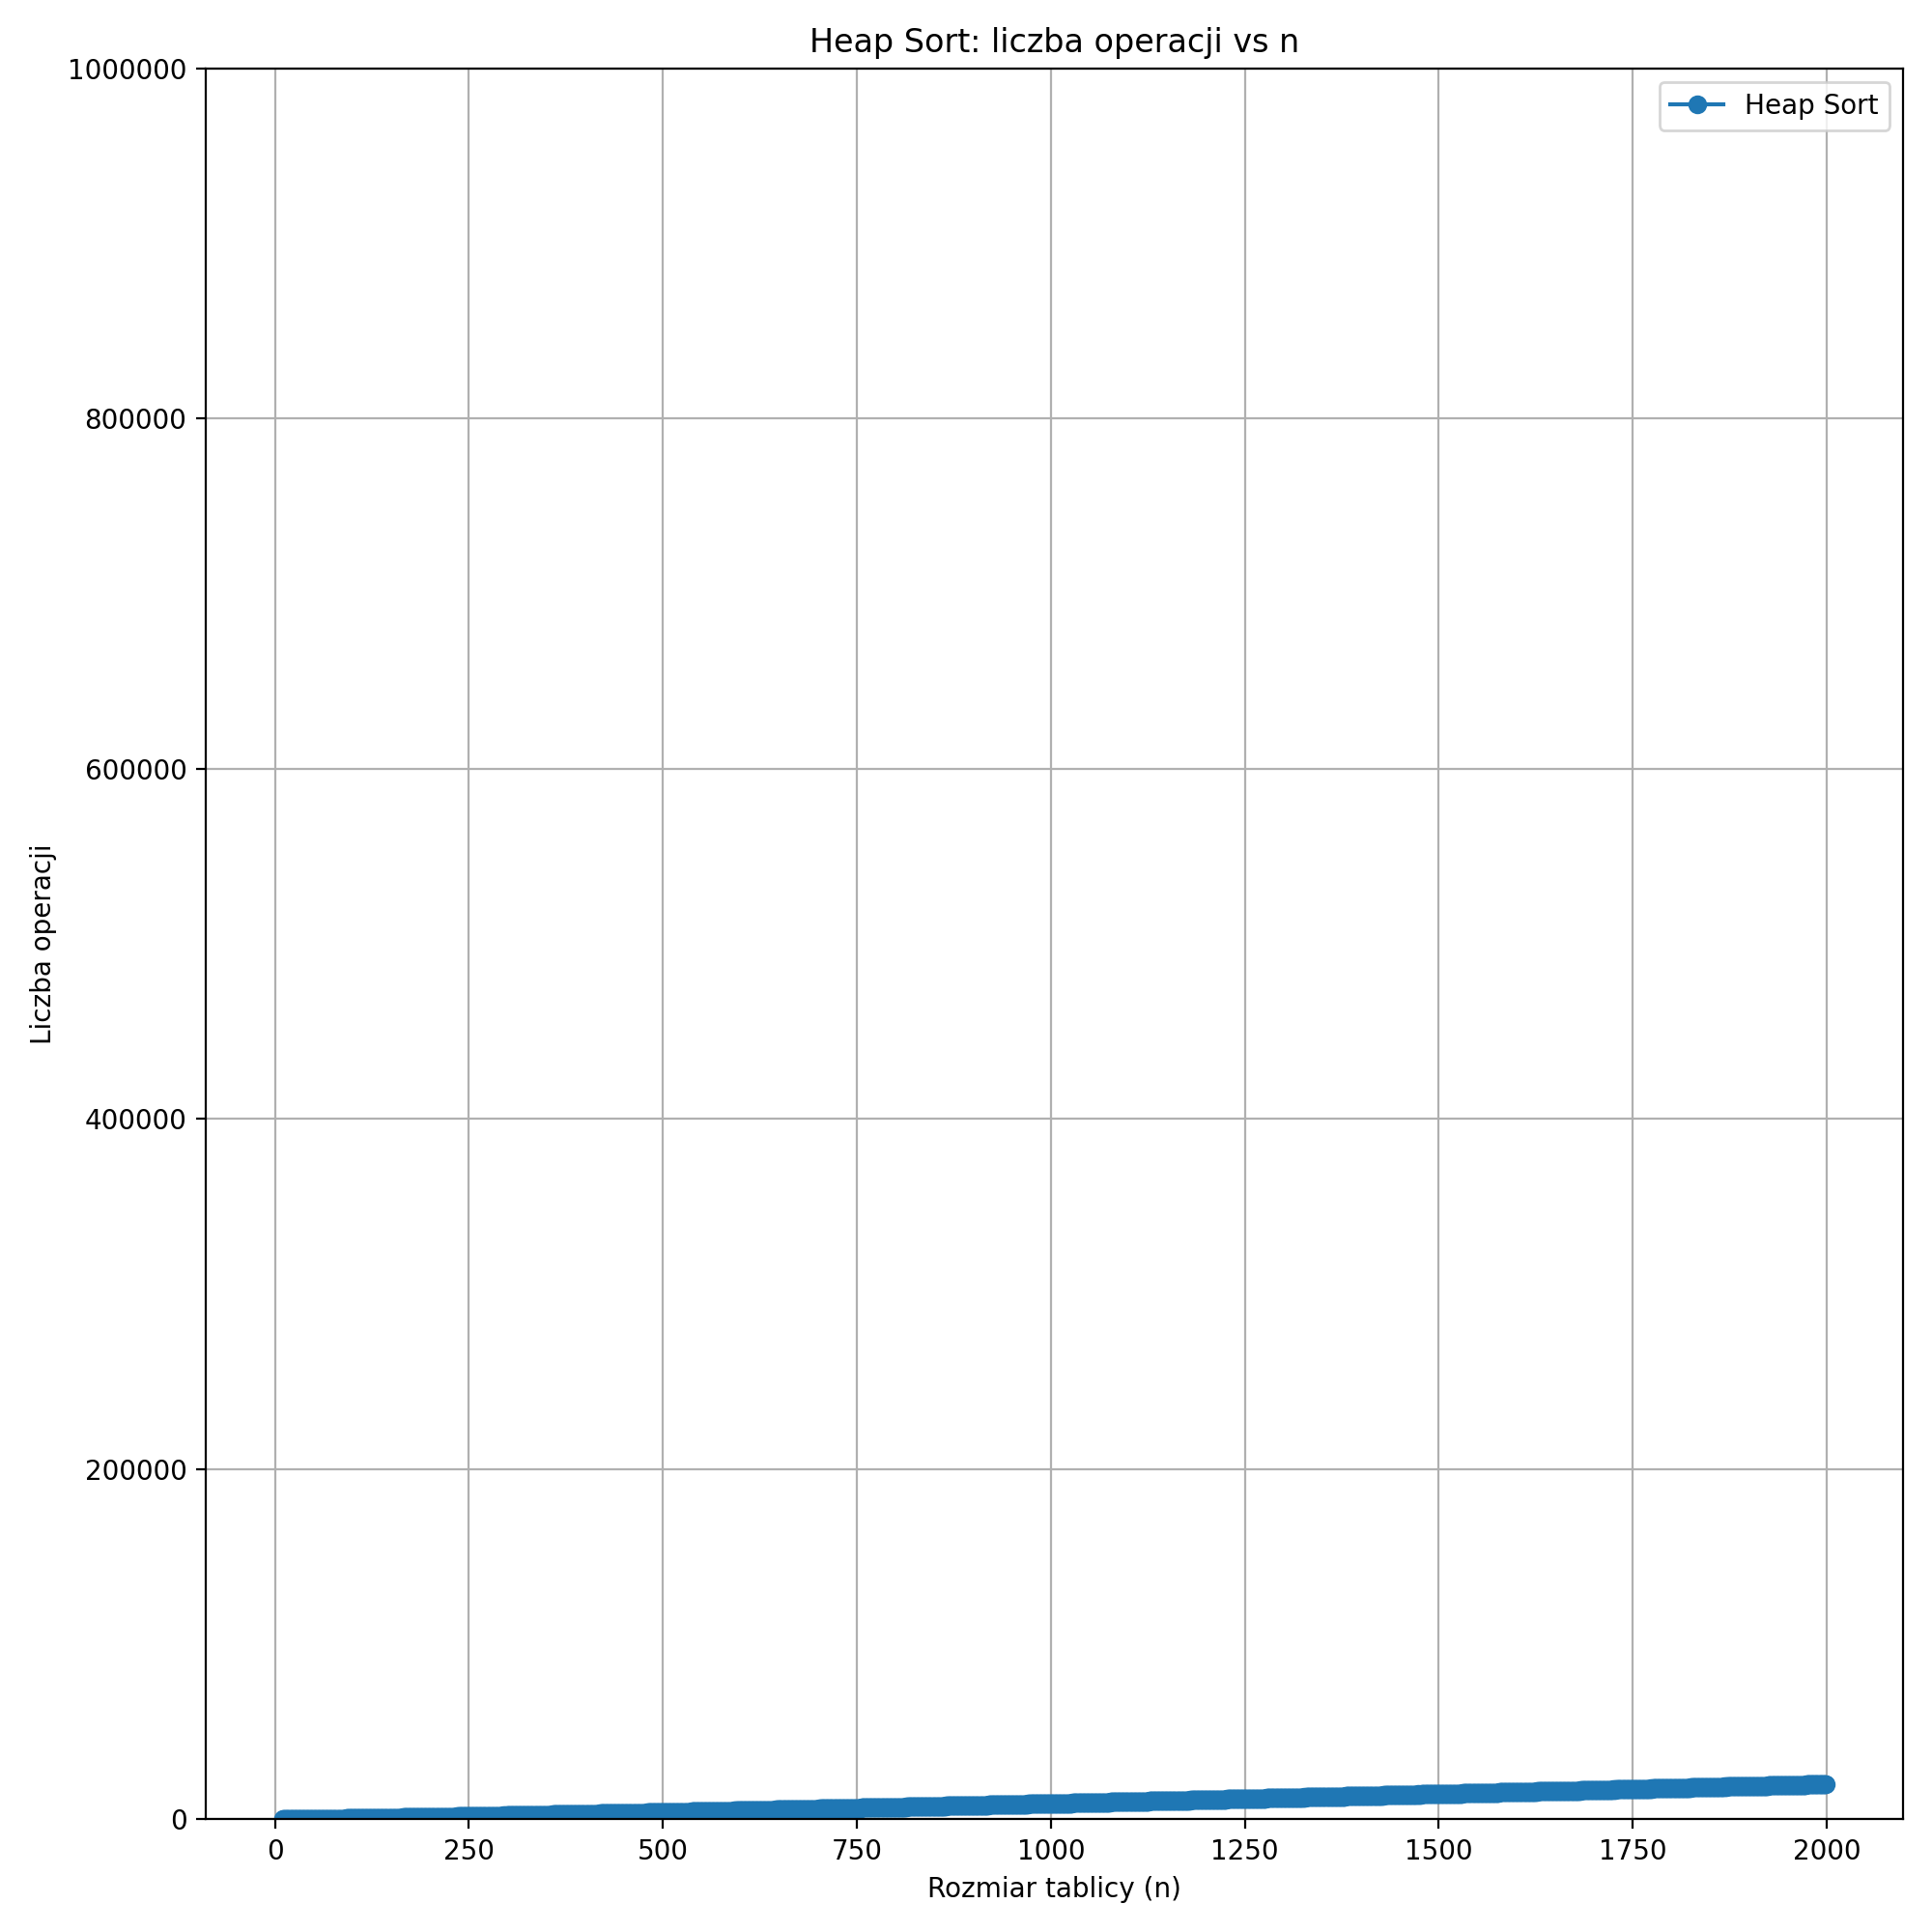
\includegraphics[width=\linewidth]{heap_sort.png}
    \caption{Heap Sort}
  \end{subfigure}
  \begin{subfigure}{.32\textwidth}
    \centering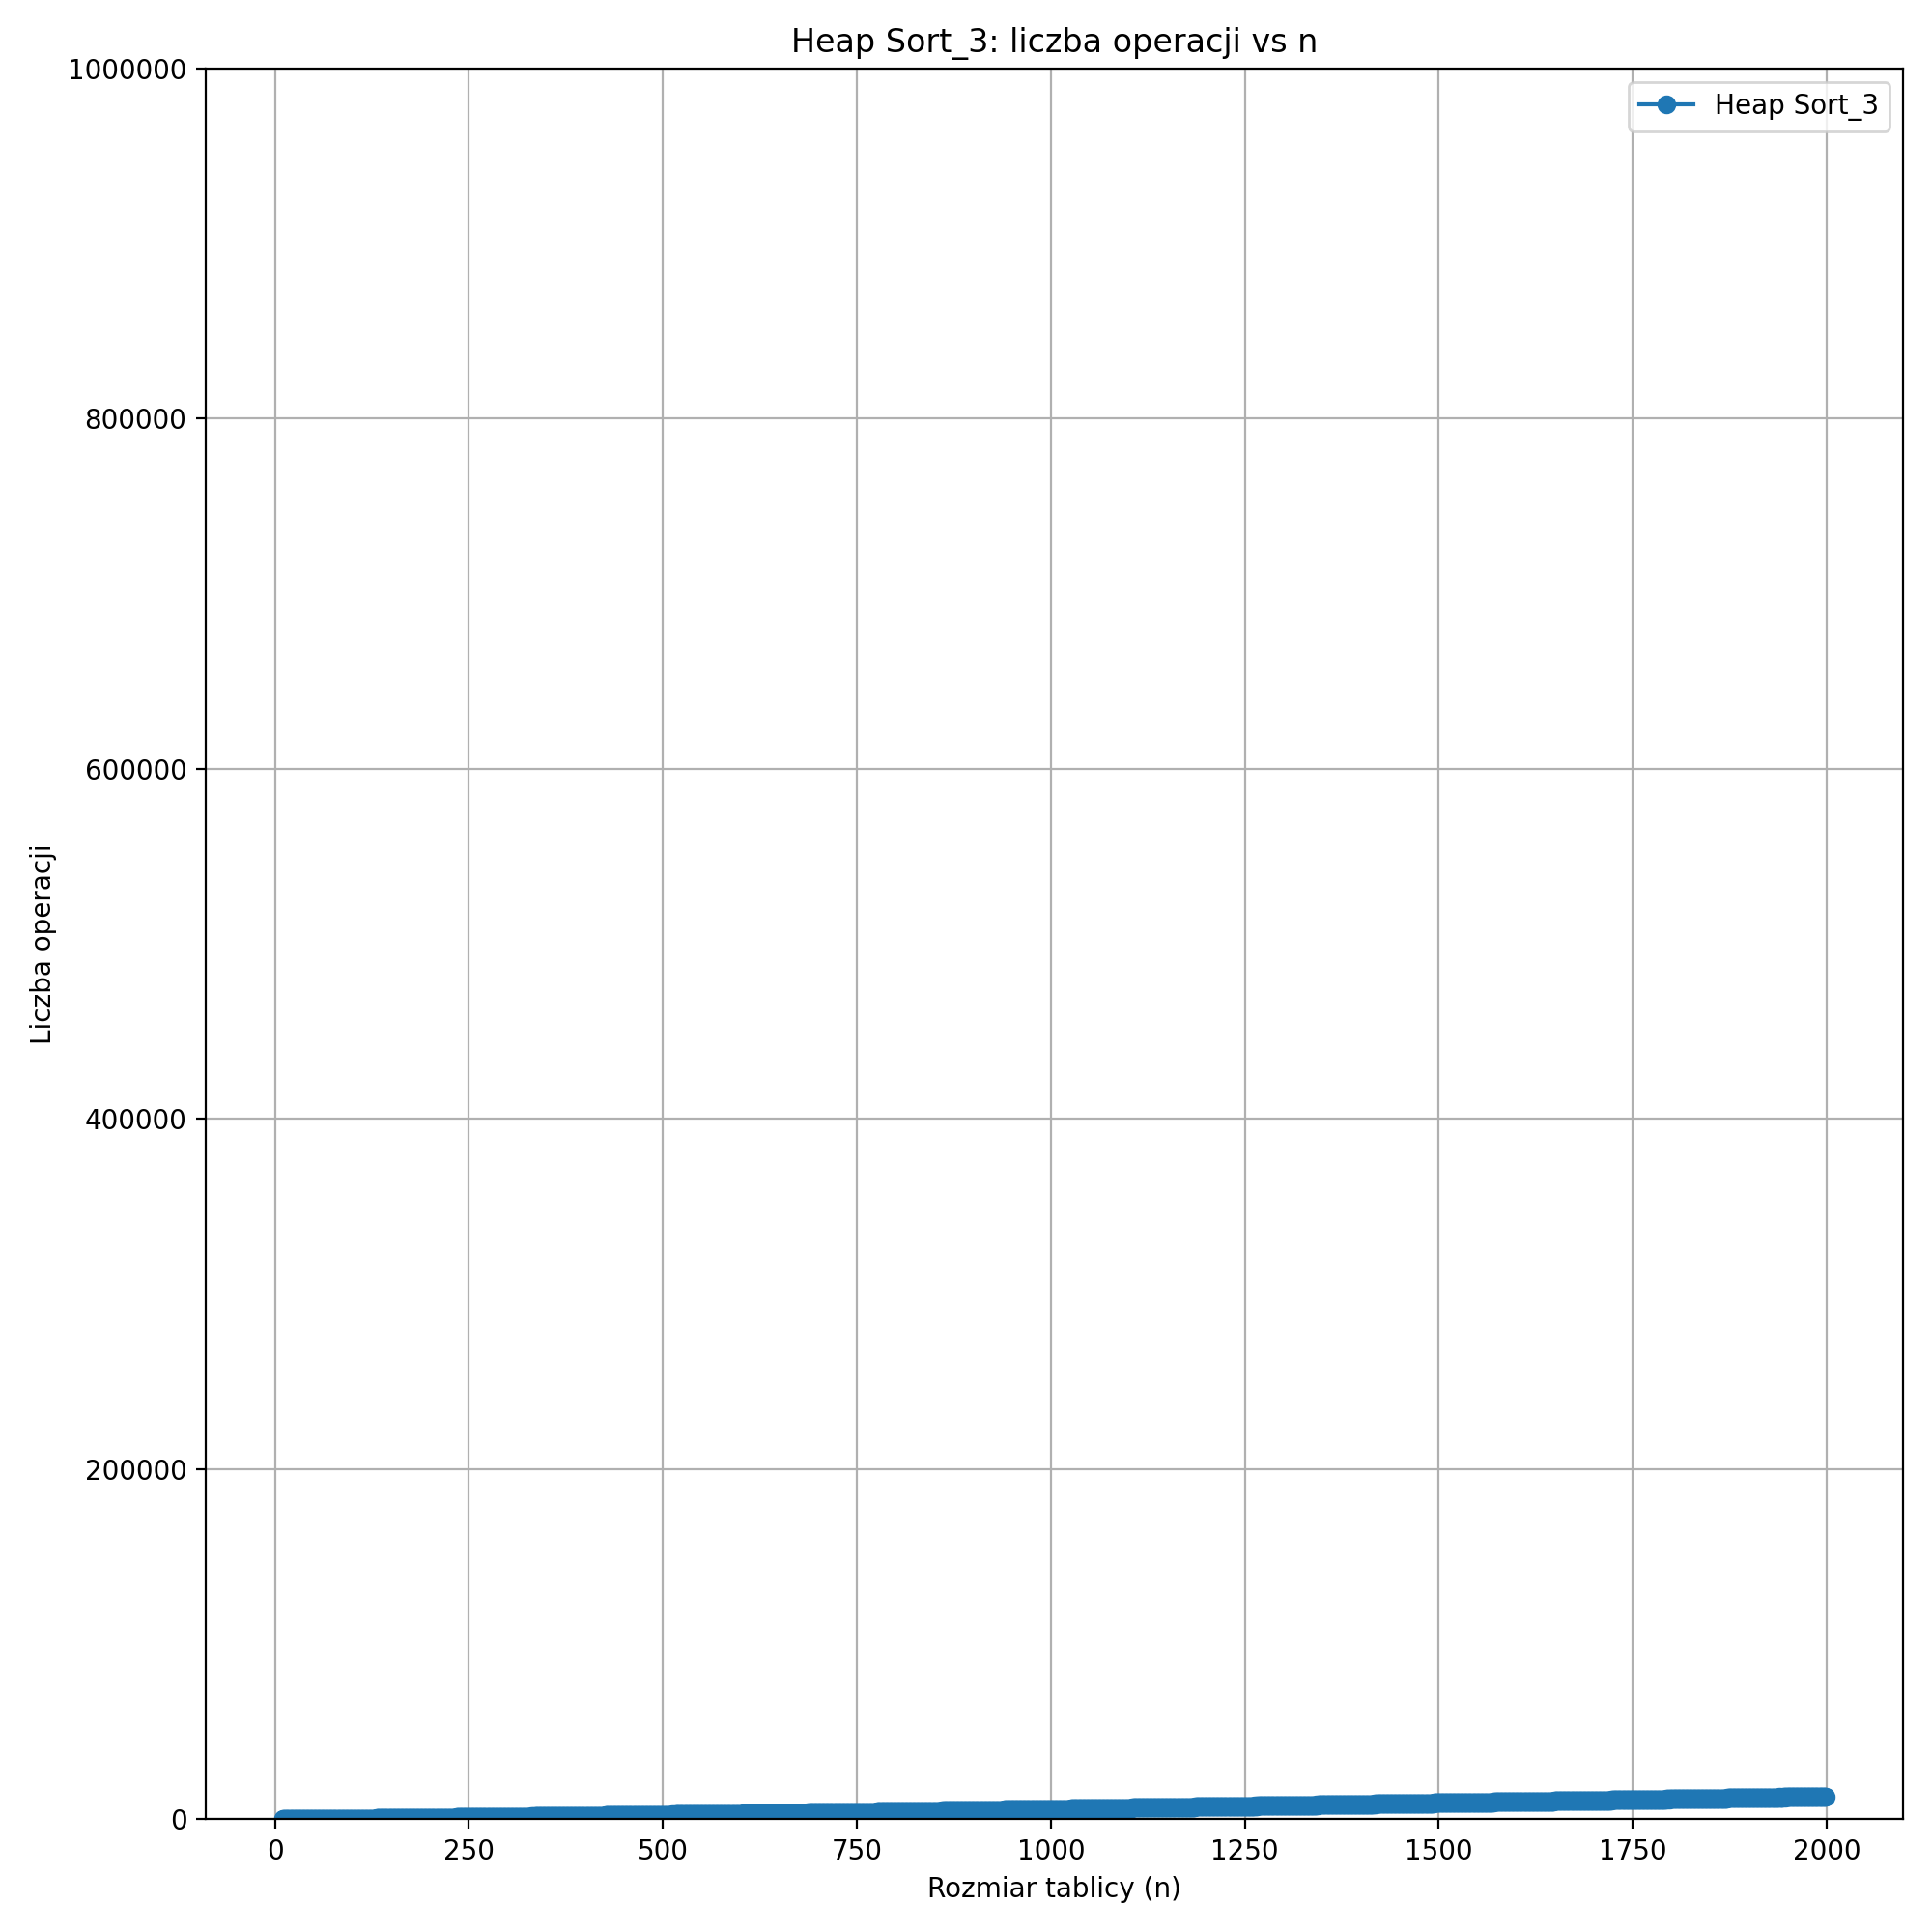
\includegraphics[width=\linewidth]{heap_sort_3.png}
    \caption{Heap Sort 3}
  \end{subfigure}
  \caption{Mini-wykresy: liczba operacji w funkcji $n$ dla każdego algorytmu.}
\end{figure}

\subsection{Tabela porównawcza złożoności i własności}
\begin{center}
\begin{tabular}{@{}lcccc@{}}
\toprule
Algorytm & Złożoność średnia & Złożoność pesymistyczna \\
\midrule
Insertion Sort & $O(n^2)$ & $O(n^2)$ \\
Insertion Sort Pairs & $O(n^2)$ & $O(n^2)$ \\
Merge Sort & $O(n\log n)$ & $O(n\log n)$  \\
Merge Sort 3 & $O(n\log n)$ & $O(n\log n)$  \\
Heap Sort & $O(n\log n)$ & $O(n\log n)$  \\
Heap Sort 3 & $O(n\log n)$ & $O(n\log n)$  \\
\bottomrule
\end{tabular}
\end{center}

\subsection{Komentarz do wyników}
\begin{itemize}
  \item \textbf{Insertion vs Insertion Pairs:} Obie krzywe rosną kwadratowo; wariant parowy redukuje liczbę przesunięć o stały czynnik, ale nie zmienia rzędu złożoności.
  \item \textbf{Merge Sort klasyczny vs Merge Sort 3:} Wariant trójdzielny osiąga \emph{nieco mniej} operacji dla dużych $n$ (mniej poziomów rekurencji), ale cena to bardziej skomplikowane scalanie.
  \item \textbf{Heap Sort binarny vs Heap Sort ternarny:} Kopiec trójdzielny ma mniejszą wysokość, jednak \texttt{heapify} musi porównać do trzech dzieci. W praktyce różnice są niewielkie; dla naszych danych \emph{Heap Sort 3} zwykle wykonuje mniej operacji.
\end{itemize}

\section{Wnioski}
\begin{enumerate}
  \item Dla dużych $n$ należy preferować algorytmy $O(n\log n)$: \emph{Merge Sort} i \emph{Heap Sort}. Wśród nich warianty modyfikowane do trójek bywają korzystne, ale zysk zależy od tego czy liczymy operacji oprócz przepisywań.
  \item \emph{Insertion Sort} pozostaje dobrym wyborem dla bardzo małych lub prawie posortowanych danych; wariant wstawiania parami może ograniczyć liczbę przesunięć, lecz nie przełamuje bariery $O(n^2)$.
  \item Zliczanie elementarnych operacji potwierdziło trendy teoretyczne: przebiegi dla \emph{Merge}/\emph{Heap} są bliskie $n\log n$, a dla \emph{Insertion} — kwadratowe.
\end{enumerate}

\end{document}
